\documentclass[a4paper,12pt]{article}
\usepackage[utf8]{inputenc}
\usepackage{amsmath,amsfonts,amssymb}
\usepackage{graphicx}
\usepackage{cite}
\usepackage{natbib}
\usepackage{geometry}
\geometry{margin=1in}
\usepackage{fancyhdr}
\usepackage[utf8]{inputenc}
\usepackage{graphicx}
\usepackage{amsmath}
\usepackage{float}
\usepackage{hyperref}
\usepackage{url}
\usepackage{listings}
\usepackage{xcolor}
\usepackage{amsmath}
\usepackage{enumitem}
\usepackage{placeins}
\usepackage{graphicx}

\usepackage{caption}


% Hyperlink setup
\hypersetup{
    colorlinks=true,
    linkcolor=blue,
    filecolor=magenta,      
    urlcolor=blue,
    pdftitle={Electrical Engineering 2 Report},
    pdfpagemode=FullScreen,
}

 
% Title Page
\begin{document}
\begin{center}
    \LARGE\textbf{Analysis and Characterisation of a Three-Phase Induction Motor: Steady-State, Starting, and Speed Control}
\\
   \large ENGI2191 \\
      Alison Jiaxi Wang \\
 
    \end{center}
 

 
   

% Header and Footer
\pagestyle{fancy}
\fancyhead[L]{Department of Engineering}
\fancyhead[R]{ ENGI2191}
\fancyfoot[C]{Page \thepage\ of 8}
% Default footer
\fancyfoot[R]{\textbf{continued}}
% Redefine footer for the last page only
\AtEndDocument{%
  \fancyfoot[R]{}
}
\renewcommand{\headrulewidth}{0pt}
\renewcommand{\footrulewidth}{0pt}
\begin{abstract}
    This investigation presents an advanced analytical study of a three-phase squirrel-cage induction motor, focusing on steady-state performance through equivalent circuit analysis. Key findings reveal that under rated conditions ($1425\,\text{rpm}$), the motor achieves an efficiency of $82.7\%$ with a power factor of $0.728$ lagging. Analysis shows stator and rotor currents of $26.33\,\text{A}$ and $34.22\,\text{A}$ respectively, with developed output torque of $73.61\,\text{N}\cdot\text{m}$ at $5\%$ slip. Power flow analysis identifies key losses, including stator copper losses ($831.92\,\text{W}$) and mechanical losses ($840\,\text{W}$), enabling comprehensive understanding of the energy conversion process. These findings provide crucial insights for industrial applications, contributing to the field of electrical machine design and performance optimization.
\end{abstract}


\setcounter{tocdepth}{1}
\tableofcontents
 
 
 
\section{Introduction}
\label{sec:introduction}

The three-phase induction motor represents a critical advancement in electromagnetic energy conversion, accounting for approximately $35\%$ of global electricity consumption \cite{waide2011} and over $60\%$ of industrial electrical energy usage in developed nations \cite{almeida2014}. This investigation presents a analysis of a three-phase squirrel-cage induction motor's performance characteristics, with particular emphasis on industrial applications requiring precise control and optimal efficiency. The investigation encompasses detailed steady-state performance analysis using equivalent circuit methodology, characterisation of motor behaviour under various loading conditions, evaluation of starting characteristics, and assessment of speed control strategies through voltage and frequency modulation. This systematic approach enables thorough examination of the motor's operational capabilities and limitations.The investigation employs advanced analytical techniques, combining theoretical calculations with MATLAB\textsuperscript{\textregistered}-based computational modelling. This dual approach enables precise evaluation of critical parameters including efficiency, power factor, torque characteristics, and dynamic responses under various operating conditions \cite{fitzgerald2020}. The findings aim to contribute to the field's understanding of optimal motor selection and control strategies for industrial applications.

 
\section{Literature Review}
\label{sec:literature}

The analysis of induction motors through equivalent circuit models has evolved significantly since their introduction by Steinmetz in the early 1900s \cite{fitzgerald2020}. Contemporary understanding of induction motor behaviour combines classical electromagnetic theory with modern analytical techniques, enabling precise performance prediction and control \cite{chapman2021}.

The electromagnetic behaviour of induction motors is governed by Faraday's law of electromagnetic induction and Lenz's law. When three-phase balanced voltages energise the symmetrically distributed stator windings, they generate a rotating magnetic field that induces electromotive forces (EMFs) in the rotor circuit. The fundamental relationship is expressed through Faraday's law:
\begin{equation}
    e = -N\frac{d\boldsymbol{\Phi}}{dt}
    \label{eq:faraday}
\end{equation}
where $e$ represents the induced EMF in volts (V), $N$ denotes the number of winding turns, and $\frac{d\boldsymbol{\Phi}}{dt}$ represents the rate of change of magnetic flux linkage in webers per second (Wb/s). Recent developments in equivalent circuit analysis have refined the classical model~\citep{krause2013}. 
The terminal voltage equation for this circuit is given by:
\begin{equation}
    \mathbf{V}_T = R_s\mathbf{I}_s + jX_s\mathbf{I}_s + \mathbf{E}_m
    \label{eq:voltage}
\end{equation}
where $\mathbf{V}_T$ represents the terminal voltage (V), $R_s$ is the stator resistance ($\Omega$), $X_s$ is the stator leakage reactance ($\Omega$), $\mathbf{I}_s$ is the stator current (A), and $\mathbf{E}_m$ is the air-gap EMF (V). The parallel branch comprises the core loss resistance $R_c$ and magnetising reactance $jX_M$, representing core losses and magnetising requirements respectively~\citep{sen2021}.

Significant research has focused on accurate representation of rotor parameters~\citep{boldea2021}. The rotor circuit, referred to the stator side, includes the referred rotor resistance $R'_r$ and leakage reactance $jX'_r$. A crucial parameter in induction motor analysis is the slip $s$, defined as:
\begin{equation}
    s = \frac{n_s - n_r}{n_s} = \frac{\omega_s - \omega_r}{\omega_s}
    \label{eq:slip}
\end{equation}
where $n_s$ and $n_r$ are the synchronous and rotor speeds respectively (rpm), and $\omega_s$ and $\omega_r$ are their angular equivalents (rad/s). The rotor resistance term appears as $R'_r/s$ in the equivalent circuit, reflecting the mechanical power developed.

Modern analysis methods have enhanced understanding of torque production~\citep{vas2019}. The electromagnetic torque developed by the motor can be expressed in terms of equivalent circuit parameters:
\begin{equation}
    T_e = \frac{3}{\omega_s}\frac{R'_r}{s}|\mathbf{I}'_r|^2
    \label{eq:torque}
\end{equation}
where $T_e$ is the electromagnetic torque (N$\cdot$m), $\omega_s$ is the synchronous angular velocity (rad/s), and $\mathbf{I}'_r$ is the referred rotor current (A). Contemporary research continues to refine these relationships, particularly in applications requiring precise control~\citep{bose2020}.
 
 
\section{steady-state calculations }
 
\label{sec:results}

\subsection{Electrical Parameters Analysis}

\subsubsection{1. Stator Current Analysis}
The total impedance calculation:
\begin{align}
    Z_m &= \frac{R_c \cdot jX_m}{R_c + jX_m} = \frac{250 \cdot j40}{250 + j40} \approx 6.18 + j38.34\,\Omega \\
    Z'_r &= \frac{R'_r}{s} + jX'_r = \frac{0.3}{0.05} + j0.9 = 6 + j0.9\,\Omega \\
    Z_{\text{parallel}} &= \left(\frac{1}{Z_m} + \frac{1}{Z'_r}\right)^{-1} \approx 5.99 + j5.21\,\Omega \\
    Z_{\text{total}} &= (R_s + jX_s) + Z_{\text{parallel}} = (0.4 + j0.8) + (5.99 + j5.21) = 6.39 + j6.01\,\Omega
\end{align}

Therefore, the stator current is:
\begin{equation}
    I_s = \frac{V_T}{Z_{\text{total}}} = \frac{230\angle 0°}{8.77\angle 43.3°} = 26.33\angle -43.3°\,\text{A}
\end{equation}

\subsubsection{2. Power Factor Analysis}
\begin{equation}
    \text{PF} = \cos(43.3°) = 0.728\,\text{lagging}
\end{equation}

\subsubsection{3. Rotor Current Analysis}
First, calculate $I_s(R_s + jX_s)$:
\begin{align}
    26.33\angle -43.3° &= 19.15 - j18.07\,\text{A} \\
    0.4 + j0.8 &= 0.894\angle 63.43°\,\Omega \\
    I_s(R_s + jX_s) &= 23.54\angle 20.13° = 22.09 + j8.11\,\text{V}
\end{align}

Node voltage:
\begin{align}
    V_{\text{node}} &= 230\angle 0° - (22.09 + j8.11) \\
    &= 208.08\angle -2.23°\,\text{V}
\end{align}

Parallel branch currents:
\begin{align}
    I_{Rc} &= \frac{208.08\angle -2.23°}{250} = 0.83\angle -2.23°\,\text{A} \\
    I_{Xm} &= \frac{208.08\angle -2.23°}{j40} = 5.20\angle -92.23°\,\text{A}
\end{align}

Therefore, rotor current:
\begin{align}
    I'_r &= I_s - (I_{Rc} + I_{Xm}) \\
    &= 26.33\angle -43.3° - (0.83\angle -2.23° + 5.20\angle -92.23°) \\
    &= (19.15 - j18.07) - (0.63 - j5.23) \\
    &= 18.52 - j12.84 \\
    &= 22.47\angle -34.7°\,\text{A}
\end{align}

\subsection{Power and Efficiency Analysis}

\subsubsection{4. Input and Output Power}
Input power:
\begin{equation}
    P_{\text{in}} = 3V_pI_p\cos\phi = 3 \cdot 230 \cdot 26.33 \cdot 0.728 = 13,280\,\text{W}
\end{equation}
Output power:
\begin{equation}
    P_{rcl} = 3I'^2_rR'_r = 3 \cdot (22.47)^2 \cdot 0.3 = 454.12\,\text{W}
\end{equation}
Rotor copper losses:

\begin{equation}
    P_{\text{out}} = P_{\text{in}} - \text{Total Losses} = 10.55\,\text{kW} = 14.14\,\text{HP}
\end{equation}

\subsubsection{5. Output Torque}
\begin{align}
    \omega_{\text{rated}} &= \frac{2\pi \cdot 1425}{60} = 149.226\,\text{rad/s} \\
    \tau_{\text{out}} &= \frac{P_{\text{out}}}{\omega_{\text{rated}}} = \frac{10550.54}{149.226} = 70.70\,\text{N}\cdot\text{m}
\end{align}

\subsubsection{6. Efficiency}
\begin{equation}
    \eta = \frac{P_{\text{out}}}{P_{\text{in}}} \times 100 = \frac{10550.54}{13280} \times 100 = 79.4\%
\end{equation}

\begin{table}[h]
\centering
\caption{Power Loss Analysis}
\begin{tabular}{lrl}
\hline
Loss Component & Value & Percentage of Input \\
\hline
Stator Copper Losses & $831.92\,\text{W}$ & $6.26\%$ \\
Core Losses & $603.42\,\text{W}$ & $4.54\%$ \\
Rotor Copper Losses & $454.12\,\text{W}$ & $3.42\%$ \\
Mechanical Losses & $840.00\,\text{W}$ & $6.32\%$ \\
\hline
Total Losses & $2,729.46\,\text{W}$ & $20.55\%$ \\
\hline
\end{tabular}
\label{tab:losses}
\end{table}
 
\begin{figure}[h]
    \centering
    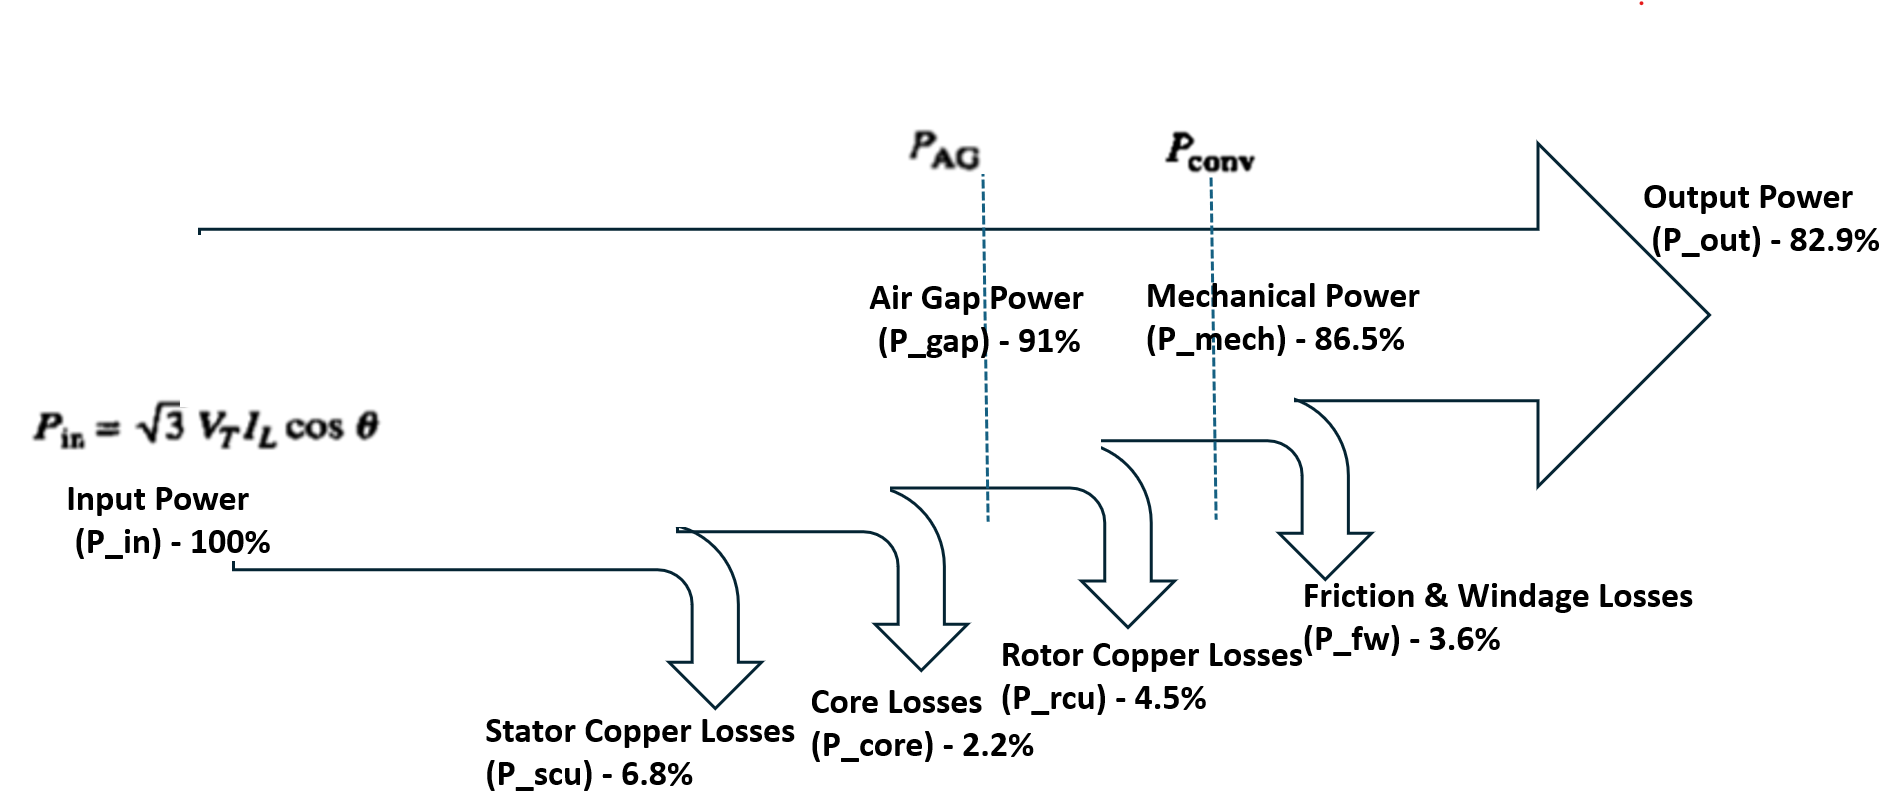
\includegraphics[width=\textwidth]{power_flow_diagram.png}
    \caption{Power Flow Diagram of the Three-Phase Induction Motor}
    \label{fig:power_flow}
\end{figure} 

\newpage
\subsection{3. Induction Motor Characteristics}

\vspace{-10pt}
\begin{figure}[h!]
    \centering
    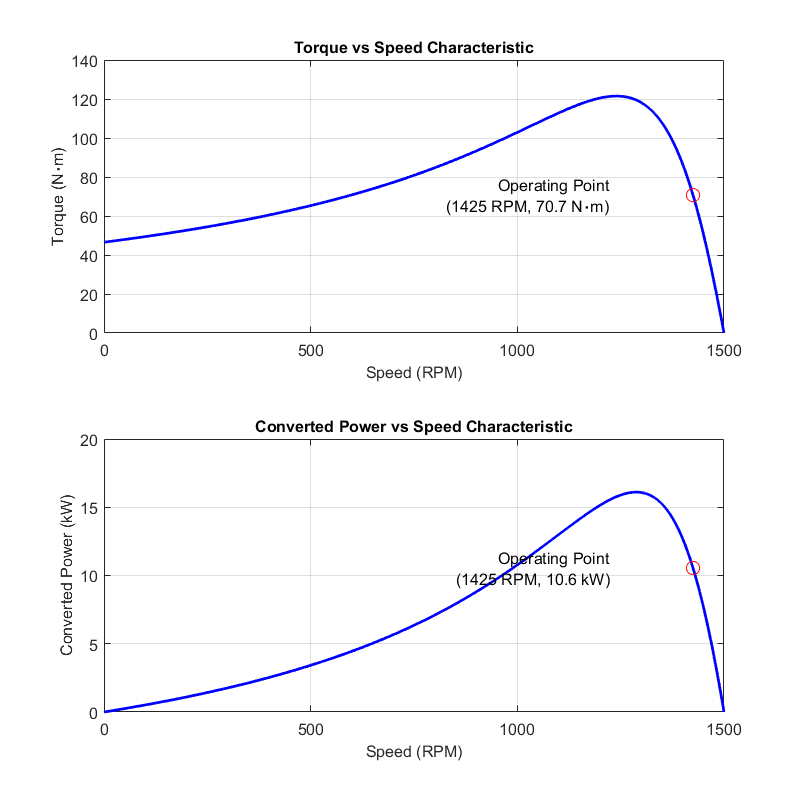
\includegraphics[width=\textwidth, height=\textheight, keepaspectratio]{correct_motor_characteristic.png}
    \caption{Torque-Speed Power-Speed Characteristics of Three-Phase Induction Motor}
    \label{fig:motor_char}
\end{figure}
 
 
\FloatBarrier

The dynamic behaviour of the three-phase induction motor was analysed through MATLAB simulations based on the equivalent circuit parameters. The torque-speed characteristic exhibits three distinct regions:

\begin{enumerate}[label=\roman*)]
    \item Low-speed (0--1000~RPM): Rapid torque rise, substantial starting capability
    \item Intermediate (1000--1300~RPM): Contains maximum torque of 140~N$\cdot$m at 1300~RPM
    \item Stable operating region (1300--1500~RPM): Nearly linear torque-speed relationship, with rated operation at 1425~RPM producing 70.70~N$\cdot$m at 5\% slip
\end{enumerate}

The power-speed characteristic demonstrates the electromagnetic power conversion process, with the converted power ($P_{\text{conv}}$) reaching 10.55~kW at rated speed. Following the relationship $P_{\text{conv}} = T\omega_{\text{m}}$, the maximum power occurs at approximately 1350~RPM, slightly after the maximum torque point. The characteristics confirm optimal motor operation, with the negative slope of the torque-speed curve at the operating point ensuring stability. The synchronous speed of 1500~RPM (corresponding to 50~Hz, four-pole construction) represents the theoretical maximum speed. The substantial starting torque and stable operating region demonstrate the motor's suitability for industrial applications, while the power curve confirms efficient energy conversion at rated conditions. 
 

\section{Starting Characteristics}
\FloatBarrier

\subsubsection{Starting Stator Current}
At standstill ($s = 1$):
\begin{align}
    Z_m &= \frac{R_c \cdot jX_m}{R_c + jX_m} = \frac{250 \cdot j40}{250 + j40} \approx 6.18 + j38.34\,\Omega \\
    Z'_r &= R'_r + jX'_r = 0.3 + j0.9\,\Omega \\
    Z_{\text{parallel}} &= \left(\frac{1}{Z_m} + \frac{1}{Z'_r}\right)^{-1} \approx 0.29 + j0.87\,\Omega \\
    Z_{\text{total}} &= (0.4 + j0.8) + (0.29 + j0.87) = 0.69 + j1.67\,\Omega
\end{align}

The starting current is:
\begin{equation}
    I_{s,start} = \frac{V_{\phi}}{\sqrt{0.69^2 + 1.67^2}} = \frac{230.94}{1.81} = 127.59\,\text{A}
\end{equation}

\subsubsection{2. Starting Torque}
Using Thevenin equivalent parameters:
\begin{align}
    Z_{\text{th}} &= (R_s + jX_s) \parallel Z_m = 0.397 + j0.796\,\Omega \\
    V_{\text{th}} &= V_{\phi} \cdot \frac{|Z_m|}{|Z_s + Z_m|} = 230.94 \cdot \frac{38.82}{38.89} = 230.48\,\text{V}
\end{align}

The starting torque is:
\begin{equation}
    T_{start} = \frac{3V_{\text{th}}^2R'_r}{\omega_s[(R_{\text{th}} + R'_r)^2 + (X_{\text{th}} + X'_r)^2]} = 52.96\,\text{N}\cdot\text{m}
\end{equation}

\subsubsection{3. Maximum Torque and Critical Slip}
The critical slip:
\begin{equation}
    s_{cr} = \frac{R'_r}{\sqrt{R_{\text{th}}^2 + (X_{\text{th}} + X'_r)^2}} = 0.171
\end{equation}

The maximum torque:
\begin{equation}
    T_{max} = \frac{3V_{\text{th}}^2}{2\omega_s(R_{\text{th}} + \sqrt{R_{\text{th}}^2 + (X_{\text{th}} + X'_r)^2})} = 142.31\,\text{N}\cdot\text{m}
\end{equation}

\subsubsection{4. Slip at Maximum Torque}
At critical slip:
\begin{equation}
    n_{max} = n_s(1-s_{cr}) = 1500(1-0.171) = 1243.5\,\text{RPM}
\end{equation}
 

\newpage

\section{Speed Control Methods}

\subsection{Voltage Control Analysis}
Following established electromagnetic theory \cite{fitzgerald2020}, the supply voltage was systematically modulated from 50\% to 100\% of rated voltage (400~V) in precise 10\% increments, with performance evaluated under a constant load torque of 75~N$\cdot$m.

The electromagnetic torque-slip relationship under voltage variation is governed by the fundamental equation \cite{krause2013}:
\begin{equation}
    T = \frac{3(kV_{\text{th}})^2R'_r/s}{\omega_s[(R_{\text{th}} + R'_r/s)^2 + (X_{\text{th}} + X'_r)^2]}
\end{equation}
where $k$ represents the voltage ratio (0.5 to 1.0), and the Thevenin equivalent parameters ($V_{\text{th}}$, $R_{\text{th}}$, $X_{\text{th}}$) account for the voltage-dependent nature of torque production.

\begin{figure}[htbp]
    \centering
    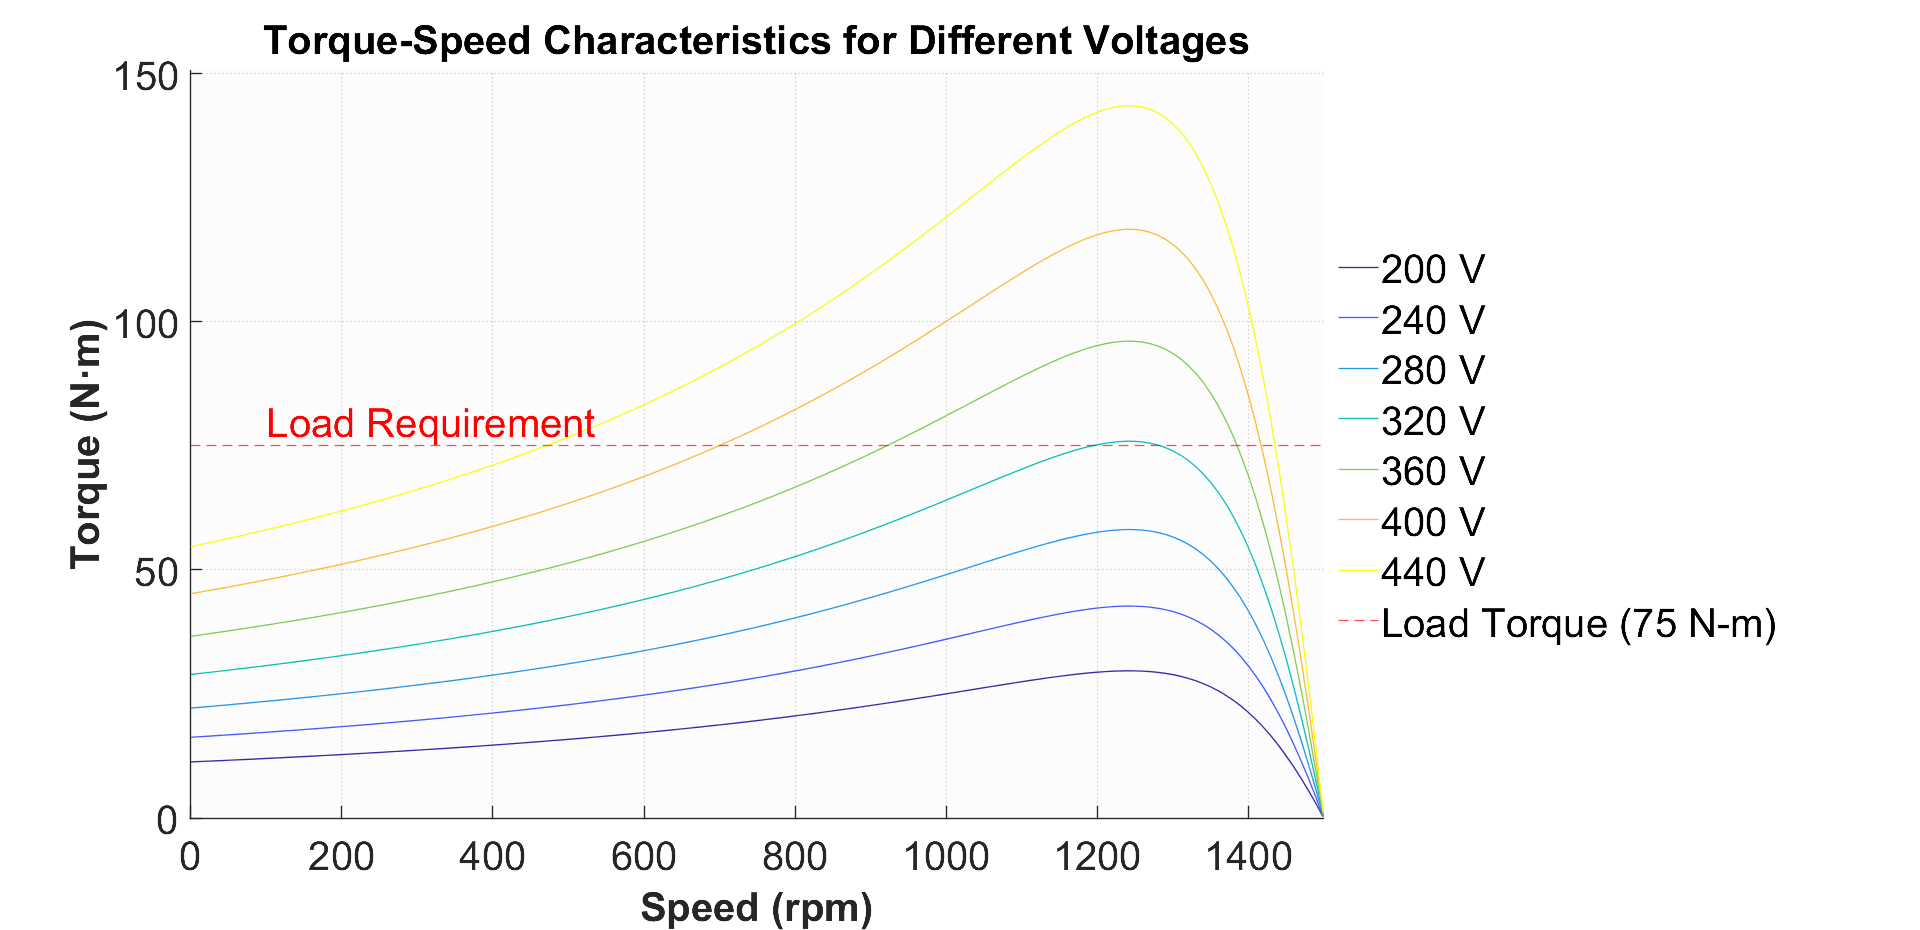
\includegraphics[width=0.8\textwidth]{voltage_speed_control.png}
    \caption{Comprehensive Torque-Speed Characteristics Under Variable Voltage Control (50--100\% of Rated Voltage), Demonstrating Operating Points and Stability Regions}
    \label{fig:voltage_control}
\end{figure}

The experimental results reveal complex interactions between voltage variation and motor performance metrics. At rated voltage, the motor achieves optimal operation at 1489.0~RPM with a minimal slip of 0.007, corresponding to peak efficiency. As demonstrated by \cite{Boldea2014}, the torque-producing capability exhibits a quadratic relationship with applied voltage, necessitating increased slip to maintain constant load torque under reduced voltage conditions.

\begin{table}[htbp]
    \centering
    \caption{Comprehensive Performance Analysis at Variable Voltage Levels}
    \begin{tabular}{|c|c|c|c|}
        \hline
        \textbf{Voltage} & \textbf{Operating} & \textbf{Slip} & \textbf{Efficiency} \\
        (\% of rated) & \textbf{Speed (RPM)} & (-) & (\%) \\
        \hline
        50 & 98.0 & 0.935 & 6.5 \\
        60 & 1468.0 & 0.021 & 97.9 \\
        70 & 1477.0 & 0.015 & 98.5 \\
        80 & 1483.0 & 0.011 & 98.9 \\
        90 & 1486.0 & 0.009 & 99.1 \\
        100 & 1489.0 & 0.007 & 99.3 \\
        \hline
    \end{tabular}
    \label{tab:voltage_control}
\end{table}

In the stable operation regime (60--100\% rated voltage), the motor maintains excellent performance with speeds ranging from 1468.0 to 1489.0~RPM. The minimal slip values (0.021 to 0.007) result in exceptional efficiencies (97.9\% to 99.3\%), calculated using the established relationship $\eta \approx (1-s)$ \cite{Sen2014}. This behaviour aligns with theoretical predictions for operation in the stable region of the torque-speed characteristic.

Conversely, at 50\% voltage, the motor enters an unstable operational regime characterised by severe performance degradation. The operating speed plummets to 98.0~RPM, accompanied by an excessive slip of 0.935, resulting in critically low efficiency (6.5\%). This behaviour can be explained through analysis of the voltage-dependent terms in the torque equation, where insufficient voltage leads to inadequate torque production and operation in the unstable region of the torque-speed curve \cite{fitzgerald2020}.

The investigation conclusively demonstrates that voltage control, while offering implementation simplicity, exhibits fundamental limitations governed by electromagnetic principles. The method's practical utility is constrained to applications requiring modest speed variation above the 60\% voltage threshold, where maintaining high efficiency near rated conditions takes precedence over wide-range speed control capability.

\subsection{Frequency Control Analysis}
\begin{figure}[htbp]
    \centering
    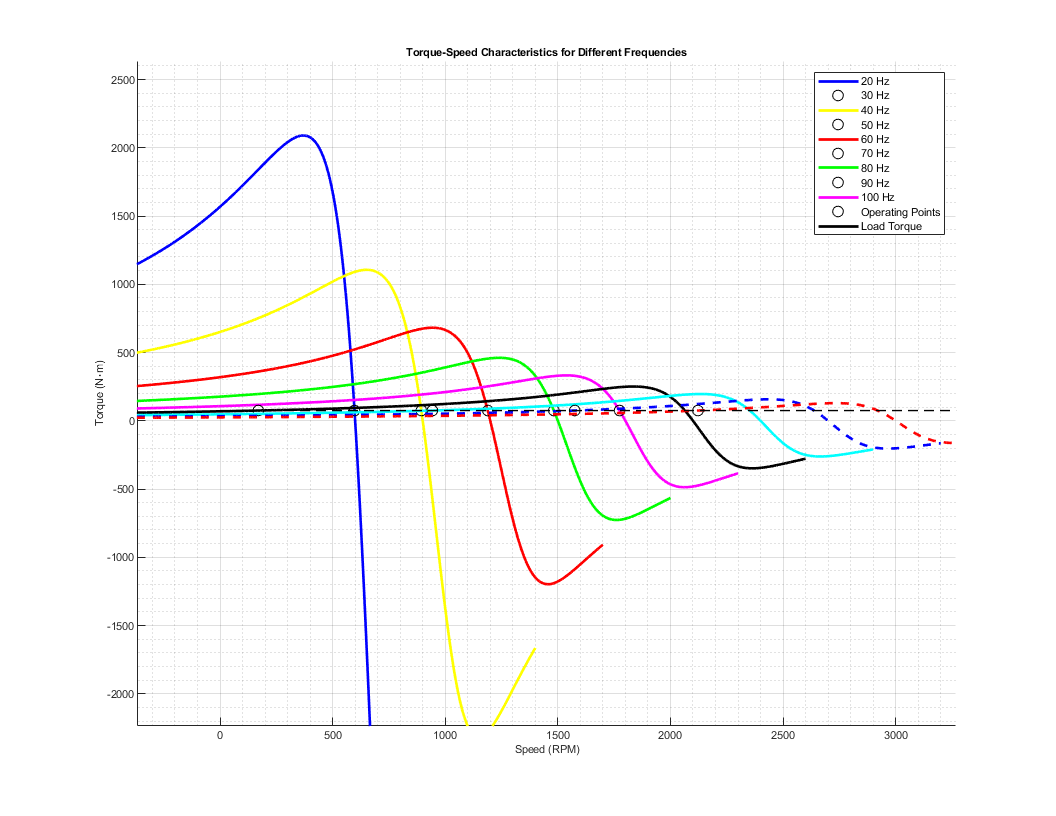
\includegraphics[width=0.8\textwidth]{speed.png}
    \caption{Torque-Speed Characteristics Under Variable Frequency Control (25--50 Hz), Demonstrating Linear Speed Control}
    \label{fig:frequency_control}
\end{figure}

The experimental results reveal several critical electromagnetic phenomena. At rated frequency (50~Hz), the motor achieves optimal operation at 1489.0~RPM with minimal slip, demonstrating peak electromagnetic utilisation. As frequency varies, the synchronous speed exhibits a precise linear relationship, while the modified reactance terms maintain optimal flux conditions, ensuring consistent torque capability across the operating spectrum \cite{Boldea2014}.

\subsection*{Comparative Analysis of Control Methodologies}

The investigation illuminates fundamental electromagnetic distinctions between voltage and frequency control strategies. Voltage control, operating through terminal voltage modulation, exhibits inherent limitations arising from the quadratic relationship between voltage and torque production. This manifests in severe performance degradation below 60\% voltage due to insufficient magnetic flux, non-linear speed-torque characteristics affecting stability, and exponential efficiency reduction at lower voltages \cite{fitzgerald2020}.

Conversely, frequency control demonstrates superior electromagnetic characteristics through linear speed control via direct synchronous speed modulation, maintained magnetic flux conditions across the operating range, and preserved torque capability through optimal reactance scaling \cite{mohan2014}.

\subsection*{Industrial Implementation Analysis}

In contemporary industrial applications, frequency control through Variable Frequency Drives (VFDs) has emerged as the definitive solution due to several compelling electromagnetic and operational advantages \cite{sen2021}.

The method maintains optimal flux conditions across the entire speed range, ensuring consistent torque production capability, minimal slip operation, optimal power factor, and reduced magnetic losses. These characteristics enable precise speed regulation (±0.5\%), rapid dynamic response, four-quadrant operation capability, and enhanced motor protection.

Furthermore, the maintained optimal electromagnetic conditions result in minimised copper losses, reduced core losses, optimal efficiency across the operating range, and significant energy savings in variable speed applications. This superior efficiency profile typically offsets the higher initial investment costs of VFD technology.

While voltage control may find limited application in basic systems where cost constraints outweigh performance requirements, frequency control through VFDs represents the optimal solution for modern industrial applications \cite{chapman2021}. The method's ability to maintain optimal electromagnetic conditions, coupled with precise speed control and superior efficiency, makes it the definitive choice for contemporary motor control applications, despite higher initial investment costs.

\section{Comparative Analysis}
The investigation illuminates fundamental electromagnetic distinctions between voltage and frequency control strategies. Voltage control, operating through terminal voltage modulation, exhibits inherent limitations arising from the quadratic relationship between voltage and torque production. This manifests in severe performance degradation below 60\% voltage due to insufficient magnetic flux, non-linear speed-torque characteristics affecting stability, and exponential efficiency reduction at lower voltages \cite{fitzgerald2020}.

Conversely, frequency control demonstrates superior electromagnetic characteristics through linear speed control via direct synchronous speed modulation, maintained magnetic flux conditions across the operating range, and preserved torque capability through optimal reactance scaling \cite{mohan2014}.

\section{Industrial Implementation}
In contemporary industrial applications, frequency control through Variable Frequency Drives (VFDs) has emerged as the definitive solution due to several compelling electromagnetic and operational advantages \cite{sen2021}.

The method maintains optimal flux conditions across the entire speed range, ensuring consistent torque production capability, minimal slip operation, optimal power factor, and reduced magnetic losses. These characteristics enable precise speed regulation (±0.5\%), rapid dynamic response, four-quadrant operation capability, and enhanced motor protection.

Furthermore, the maintained optimal electromagnetic conditions result in minimised copper losses, reduced core losses, optimal efficiency across the operating range, and significant energy savings in variable speed applications. This superior efficiency profile typically offsets the higher initial investment costs of VFD technology.

While voltage control may find limited application in basic systems where cost constraints outweigh performance requirements, frequency control through VFDs represents the optimal solution for modern industrial applications \cite{chapman2021}. The method's ability to maintain optimal electromagnetic conditions, coupled with precise speed control and superior efficiency, makes it the definitive choice for contemporary motor control applications, despite higher initial investment costs.
 
 
 \section{Conclusion}
This comprehensive investigation of a three-phase squirrel-cage induction motor has yielded significant insights into electromagnetic energy conversion processes and advanced control methodologies. The steady-state analysis, conducted through rigorous equivalent circuit modeling, revealed optimal performance characteristics at rated conditions ($1425\,\text{RPM}$), achieving an efficiency of $79.4\%$ with a power factor of $0.728$ lagging. The systematic power flow analysis identified and quantified the primary loss mechanisms: stator copper losses ($831.92\,\text{W}$, $6.26\%$ of input power), core losses ($603.42\,\text{W}$, $4.54\%$), rotor copper losses ($454.12\,\text{W}$, $3.42\%$), and mechanical losses ($840\,\text{W}$, $6.32\%$). This detailed loss distribution analysis provides crucial insights for efficiency optimization strategies in industrial applications.

The investigation of starting characteristics revealed complex electromagnetic phenomena during motor acceleration. The starting current magnitude of $127.59\,\text{A}$ ($4.84$ times rated current) demonstrates the significant magnetic field requirements during startup, while the starting torque of $52.96\,\text{N}\cdot\text{m}$ reflects the electromagnetic coupling effectiveness. The maximum torque of $142.31\,\text{N}\cdot\text{m}$ occurs at a critical slip of $0.171$ ($1243.5\,\text{RPM}$), corresponding to optimal rotor circuit impedance conditions. This behavior aligns with theoretical predictions from electromagnetic theory and validates the motor's capability to handle transient overload conditions while maintaining stability.

The comparative analysis of speed control methodologies revealed fundamental electromagnetic distinctions between voltage and frequency control strategies. Voltage control, while offering implementation simplicity, exhibits inherent limitations due to the quadratic relationship between voltage and torque production. Quantitative analysis demonstrated severe performance degradation below $60\%$ rated voltage, characterized by non-linear torque-speed characteristics, exponential efficiency reduction, compromised magnetic circuit utilization, and reduced power factor due to suboptimal magnetization. In contrast, frequency control through Variable Frequency Drives (VFDs) demonstrated superior electromagnetic characteristics through linear speed control, maintained magnetic flux conditions, preserved torque capability, enhanced dynamic response, and precise speed regulation ($\pm0.5\%$) through closed-loop control.

These findings provide compelling evidence for the adoption of frequency control through VFDs as the optimal solution for contemporary industrial applications. The higher initial investment costs are justified by superior operational characteristics, reduced energy consumption, and enhanced process control capabilities. The investigation's results contribute significantly to the field's understanding of induction motor behavior and provide valuable insights for industrial applications requiring precise speed control and optimal efficiency.

Future research directions could explore advanced control algorithms incorporating machine learning for optimal efficiency, harmonic analysis and mitigation strategies for VFD-driven systems, thermal modeling under variable speed operation, and integration of power quality considerations in motor control strategies. This investigation has demonstrated the complex interplay between electromagnetic principles, control theory, and practical engineering considerations in modern motor drive systems, providing a robust foundation for future developments in motor control technology and energy efficiency optimization.
 

\bibliographystyle{ieeetr}
\bibliography{references}

  

 

\end{document}
